%\documentclass{acmsiggraph}                     % final
%\documentclass[annualconference]{acmsiggraph}  % final (annual conference)
\documentclass[review]{acmsiggraph}            % review
%\documentclass[widereview]{acmsiggraph}        % wide-spaced review
%\documentclass[preprint]{acmsiggraph}          % preprint

%% Uncomment one of the five lines above depending on where your paper is
%% in the conference process. ``review'' and ``widereview'' are for review
%% submission, ``preprint'' is for pre-publication, and ``final'' is for
%% the version to be printed. The ``final'' variant will accept the 
%% ``annualconference'' parameter, which changes the height of the space
%% left clear for the ACM copyright information.

%% The 'helvet' and 'times' packages define the typefaces used for
%% serif and sans serif type in this document. Computer Modern Roman 
%% is used for mathematics typesetting. The scale factor is set to .92
%% to bring the sans-serif type in line with the serif type.

\usepackage[scaled=.92]{helvet}
\usepackage{times}

%% The 'graphicx' package allows for the inclusion of EPS figures.

\usepackage{graphicx}

%% use this for zero \parindent and non-zero \parskip, intelligently.

\usepackage{parskip}

%% Optional: the 'caption' package provides a nicer-looking replacement
%% for the standard caption environment. With 'labelfont=bf,'textfont=it',
%% caption labels are bold and caption text is italic.

\usepackage[labelfont=bf,textfont=it]{caption}

%% If you are submitting a paper to the annual conference, please replace 
%% the value ``0'' below with the numeric value of your OnlineID. 
%% If you are not submitting this paper to the annual conference, 
%% you may safely leave it at ``0'' -- it will not be included in the output.

\usepackage{listings}
\usepackage{alltt}
\usepackage{subfigure}
%%\usepackage[caption=false]{subfig}

%%\onlineid{paper1002}

%% Paper title.

\title{Integration of X3D Geospatial in a Data Driven Web Application}

%% Author and Affiliation (single author).

%%\author{Roy G. Biv\thanks{e-mail: roy.g.biv@aol.com}\\Allied Widgets Research}

%% Author and Affiliation (multiple authors).

\author{Michael McCann\thanks{e-mail: mccann@mbari.org}\\MBARI
\and Don Brutzman\thanks{e-mail: brutzman@nps.edu}\\Naval Postgraduate School}


%% Keywords that describe your work.

\keywords{3-D Geography, X3D, geospatial, X3D-Earth, X3DOM, PostGIS, terrain rendering, sensor web, Oceanography, data visualization}

%%%%%% START OF THE PAPER %%%%%%

\begin{document}


%%\teaser{
%%\subfigure{
%%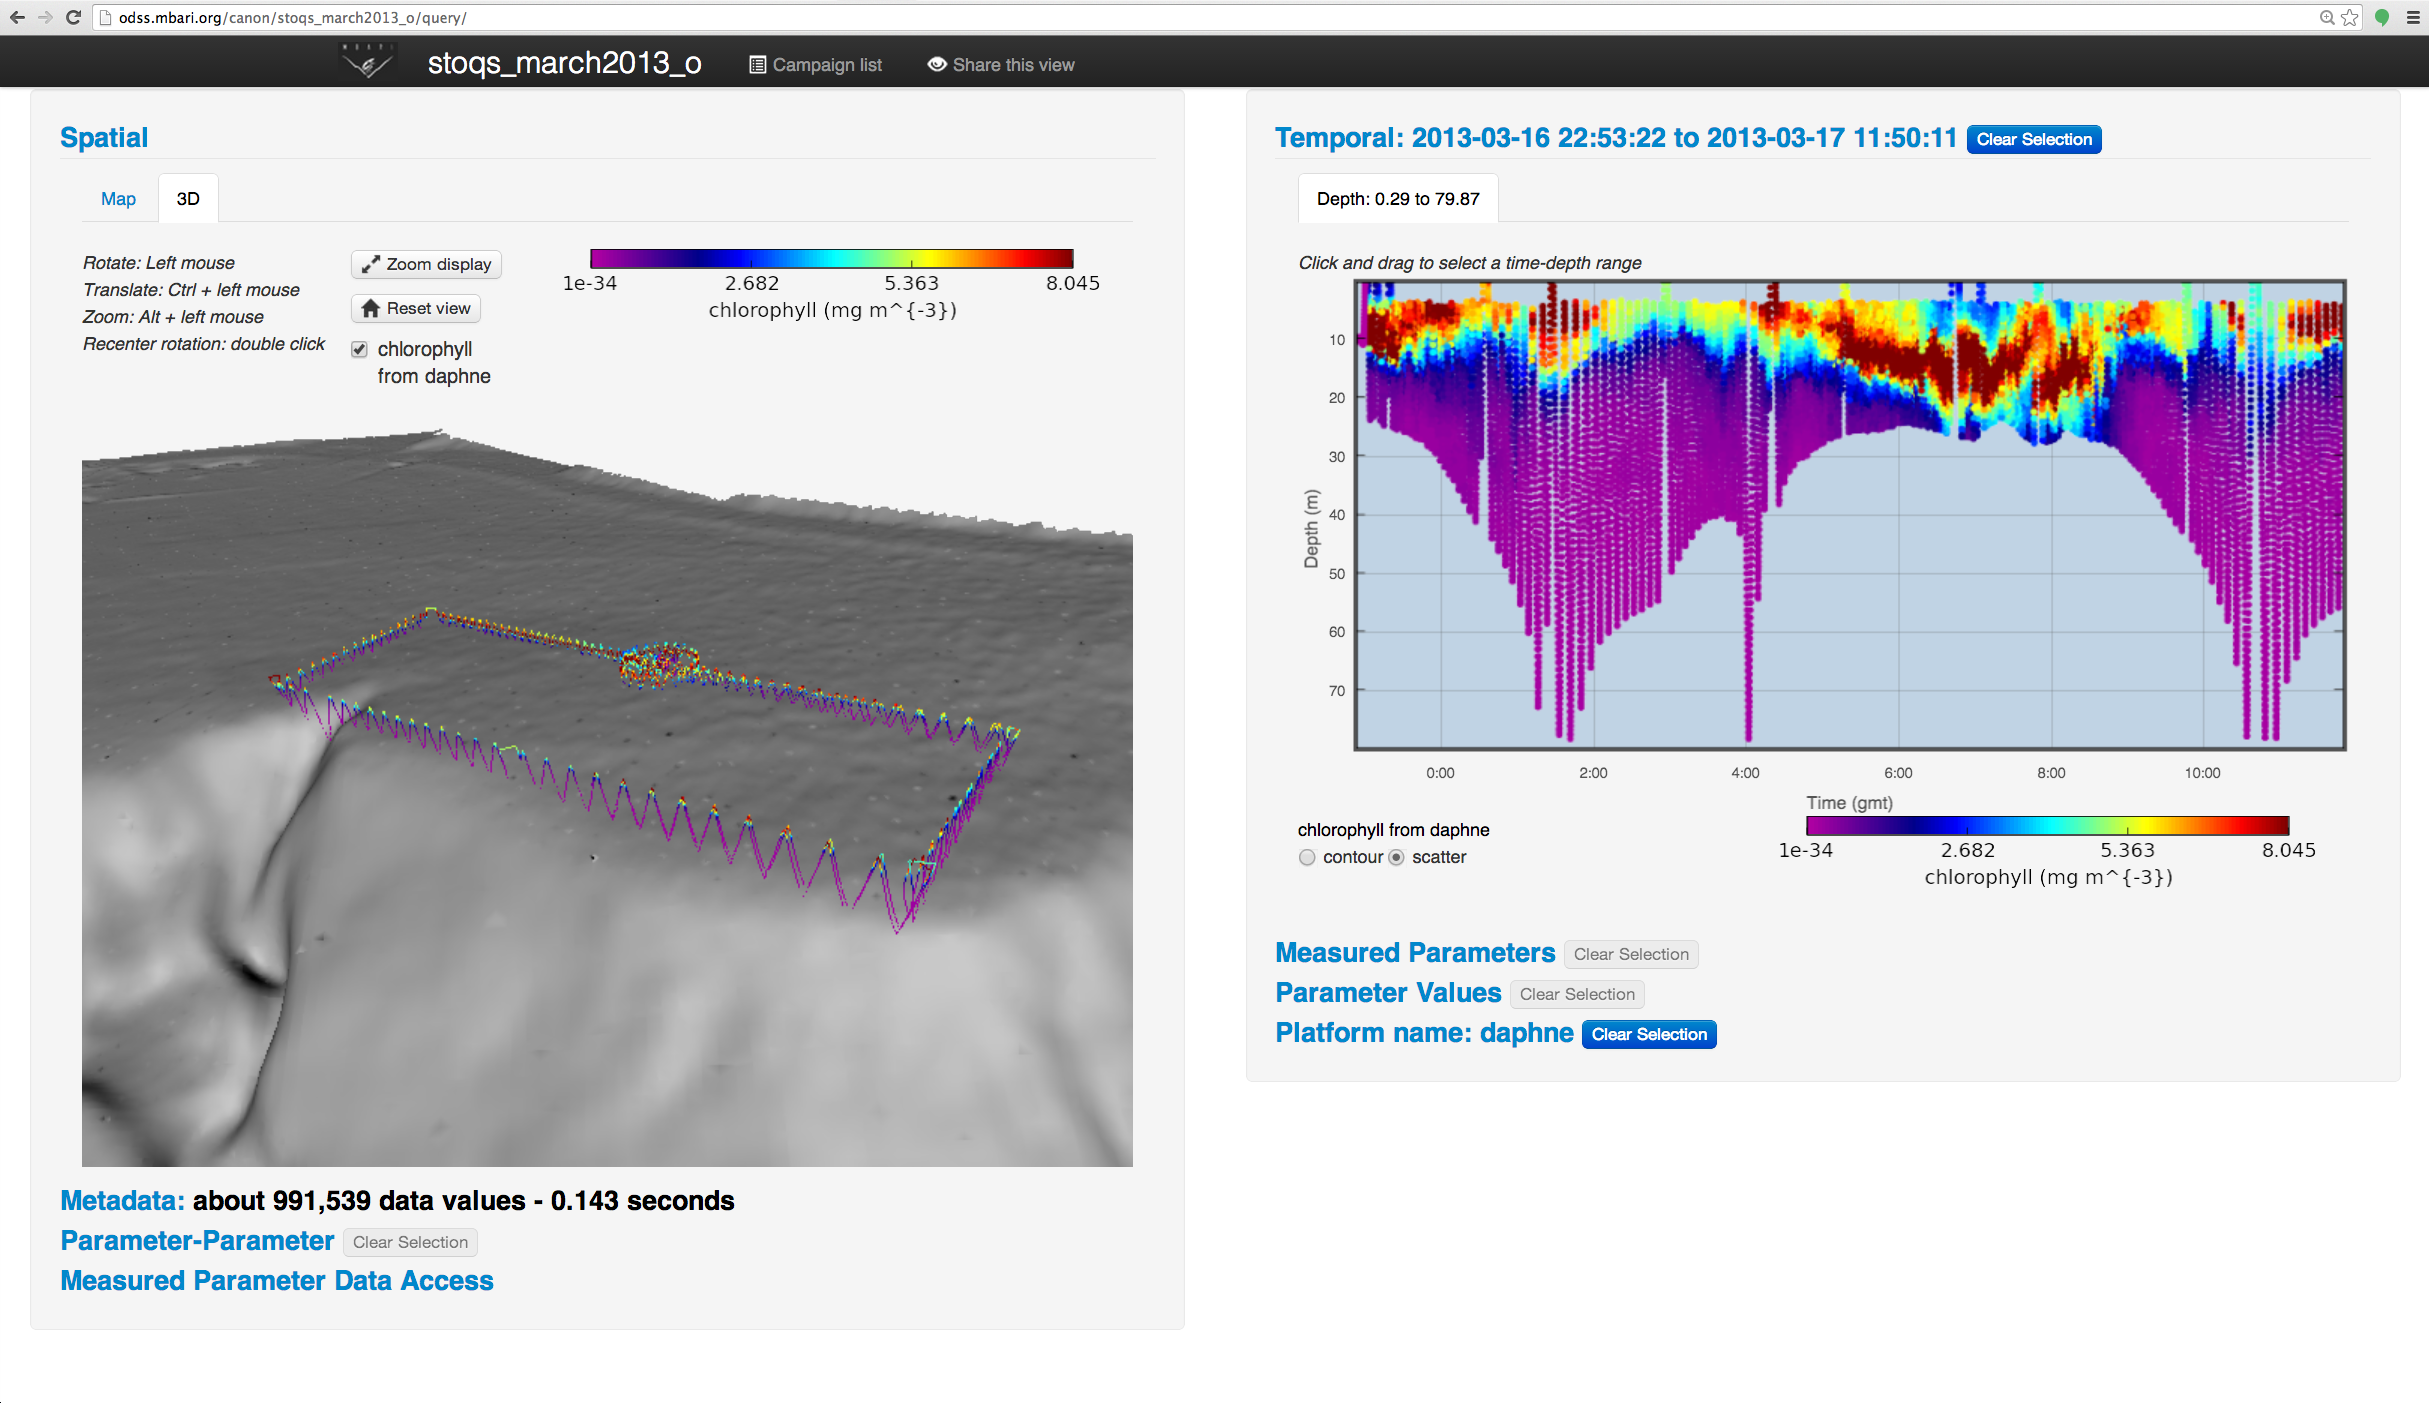
\includegraphics[height=3in]{STOQSUIscreencapture.png}
%%}
%%\label{fig:STOQSscreen_capture}
%%\caption{Screen capture of the STOQS web application showing underwater sensor data off the coast of southern California.}
%%}




%% The ``\maketitle'' command must be the first command after the
%% ``\begin{document}'' command. It prepares and prints the title block.

\maketitle

%% Abstract section.

\begin{abstract}

Efficient analysis of growing types of oceanographic observations requires new approaches in data management and visualization. The Monterey Bay Aquarium Research Institute designed the Spatial Temporal Oceanographic Query System (STOQS) to enable new capabilities for helping scientists gain insight from their data. STOQS includes a web-based graphical user interface enabling effective data exploration across all dimensions of the data collection; this interface is the platform used for integration of 3D geospatial data visualization using the X3D standard. This paper describes how the STOQS user interface uses the X3DOM to render oceanographic data and discusses what service and content standards are useful for presentation of sensor data. 


\end{abstract}

%% ACM Computing Review (CR) categories. 
%% See <http://www.acm.org/class/1998/> for details.
%% The ``\CRcat'' command takes four arguments.

\begin{CRcatlist}
  \CRcat{I.3.7}{Computing Methodologies}{Computer Graphics}{Three-Dimensional Graphics and Realism}
\end{CRcatlist}

%% The ``\keywordlist'' command prints out the keywords.
\keywordlist

\section{Introduction}

%%\copyrightspace
%% The ``\copyrightspace'' command must be the first command after the 
%% start of the first section of the body of your paper. It ensures the
%% copyright space is left at the bottom of the first column on the first
%% page of your paper.

With increased ability to acquire measurements from oceanographic platforms such as ships, moorings, drifters, gliders and autonomous underwater vehicles (AUVs), the need to efficiently access and visualize the data they collect is growing. The Monterey Bay Aquarium Research Institute has designed and built the Spatial Temporal Oceanographic Query System (STOQS) specifically to address this issue. The fundamental issue of providing efficient management and access to multidisciplinary data is addressed by embracing existing standards and employing geospatial relational database technology along with modern web frameworks to build a tool that enables deep exploration of complex data sets.

Standards are important for the durability of data archived from oceanographic measurement programs. The data are often unique and costly to collect. One of the standards used within the oceanographic community is NetCDF. It is a binary data format used commonly for gridded numerical model output and for remote sensing data. Because of its 20-plus year history of use, its flexibility, and because of its recent adoption as an Open Geospatial Consortium standard NetCDF is used for archiving of MBARI's \textit{in situ} measurement data.

The NetCDF data format (with the Climate and Forecast conventions) provide efficient data access for array data such as from numerical models because if provides indexed access to data on the coordinate dimensions. A NetCDF file performs like a mini database for data organized on a grid of longitude, latitude, depth, and time values. Retrieving spatial-temporal subsets from from multi-gigabyte array happens with a seek into the NetCDF file returning specific data values as efficiently as possible. 

\begin{figure}[htbp]
\centering
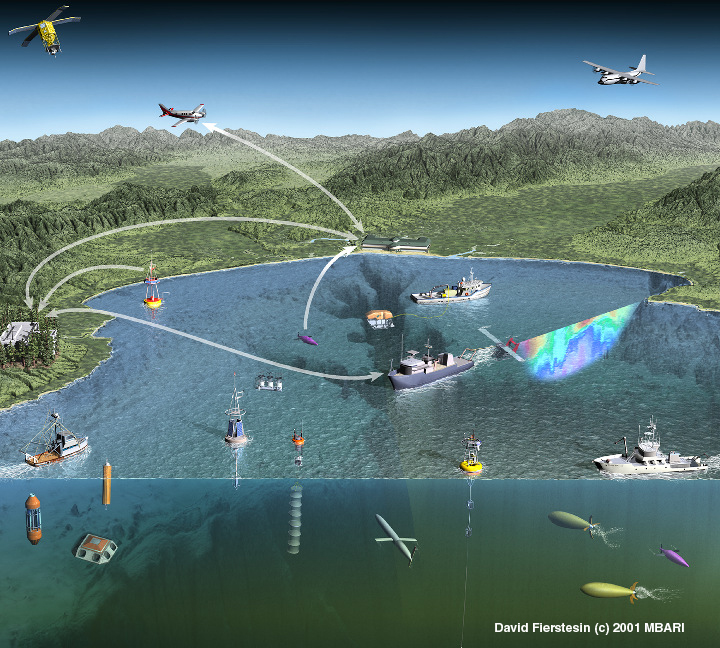
\includegraphics[width=3.3in]{MUSE_illus_pp.jpg}
\caption{Illustration of an oceanographic measurement campaign with multiple data collecting platforms.}
\label{fig:MUSE_illus_pp}
\end{figure}

This data access advantage does not exist for \textit{in situ} measurement data stored in NetCDF files. Trajectory data is increasingly being collected by a variety of new platforms. These include all the measurements taken by vehicles such as ships, drifters, gliders, and AUVs (Fig.~\ref{fig:MUSE_illus_pp}). These data are structured in NetCDF files with one coordinate dimension: time. Even though the data are distributed through space the only index into the mini-database NetCDF file is along time. There is no efficient way to retrieve specific spatial-temporal data directly from a trajectory NetCDF file. For example, if an application program needed to extract just the surface temperatures from a glider data file - where the glider samples the water column in a sawtooth pattern from 0 to 500 meters depth - it would have to read all of the data from the NetCDF file and then perform the extraction. This is a very inefficient way to access data; if the trajectory data were in a fully indexed relational database then applications can have efficient data access. This is what STOQS provides. This paper describes its architecture and a web application that provides interactive 3D visualization using standard web technology.



\section{STOQS}

STOQS has been in use at MBARI for over 3 years to help manage data collected during upper water column measurement campaigns where scientific goals center on improving our understanding of biological processes. The data consist primarily of measurements collected by moving platforms. The platforms have accurate clocks, Global Positioning Sensors and underwater inertial navigation sensors, and one or more instruments that measure parameters such as temperature, salinity, oxygen, nitrate, chlorophyll fluorescence, optical backscatter, and spectra of particle sizes. Some platforms can also capture water samples for later laboratory analysis. The typical workflow for using STOQS is:
\begin{enumerate}
\item Install the STOQS software on a Linux server 
\item Vehicles conduct their missions, collecting data 
\item Create NetCDF files of the instrument data 
\item Construct and execute a STOQS load script
\item Access and visualize data using the STOQS UI
\end{enumerate}

\subsection{Architecture}

STOQS consists of a PostgreSQL/PostGIS database, Mapserver, and Python-Django running on a server and client-side technology (jQuery, OpenLayers, Twitter Bootstrap) running in a modern web browser (Fig.~\ref{fig:STOQSArch}) . The web application provides faceted search capabilities allowing a user to quickly drill into data of interest. Data selection can be constrained by spatial, temporal, and depth selections as well as by parameter values and platform names. The web application layer also provides a REST (Representational State Transfer) Application Programming Interface allowing tools such as the Matlab stoqstoolbox to retrieve data directly from the database. The X3DOM Javascript library provides interactive 3D views of the data in browsers that support WebGL.  

\begin{figure}[htbp]
\centering
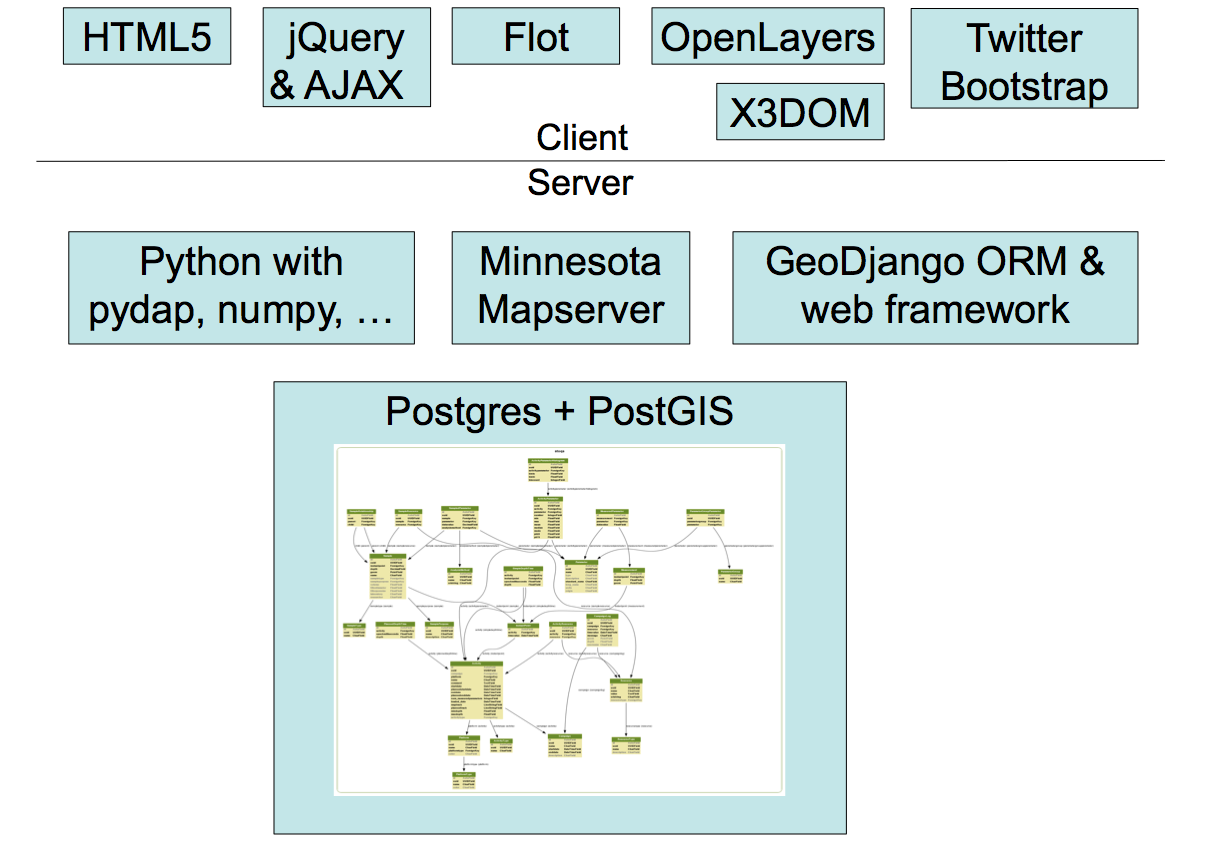
\includegraphics[width=3.3in]{STOQS_Architecture_withX3DOM.png}
\caption{Major software components that make up the STOQS platform.}
\label{fig:STOQSArch}
\end{figure}

\subsection{User Interface}

\begin{figure*}[htbp]
\centering
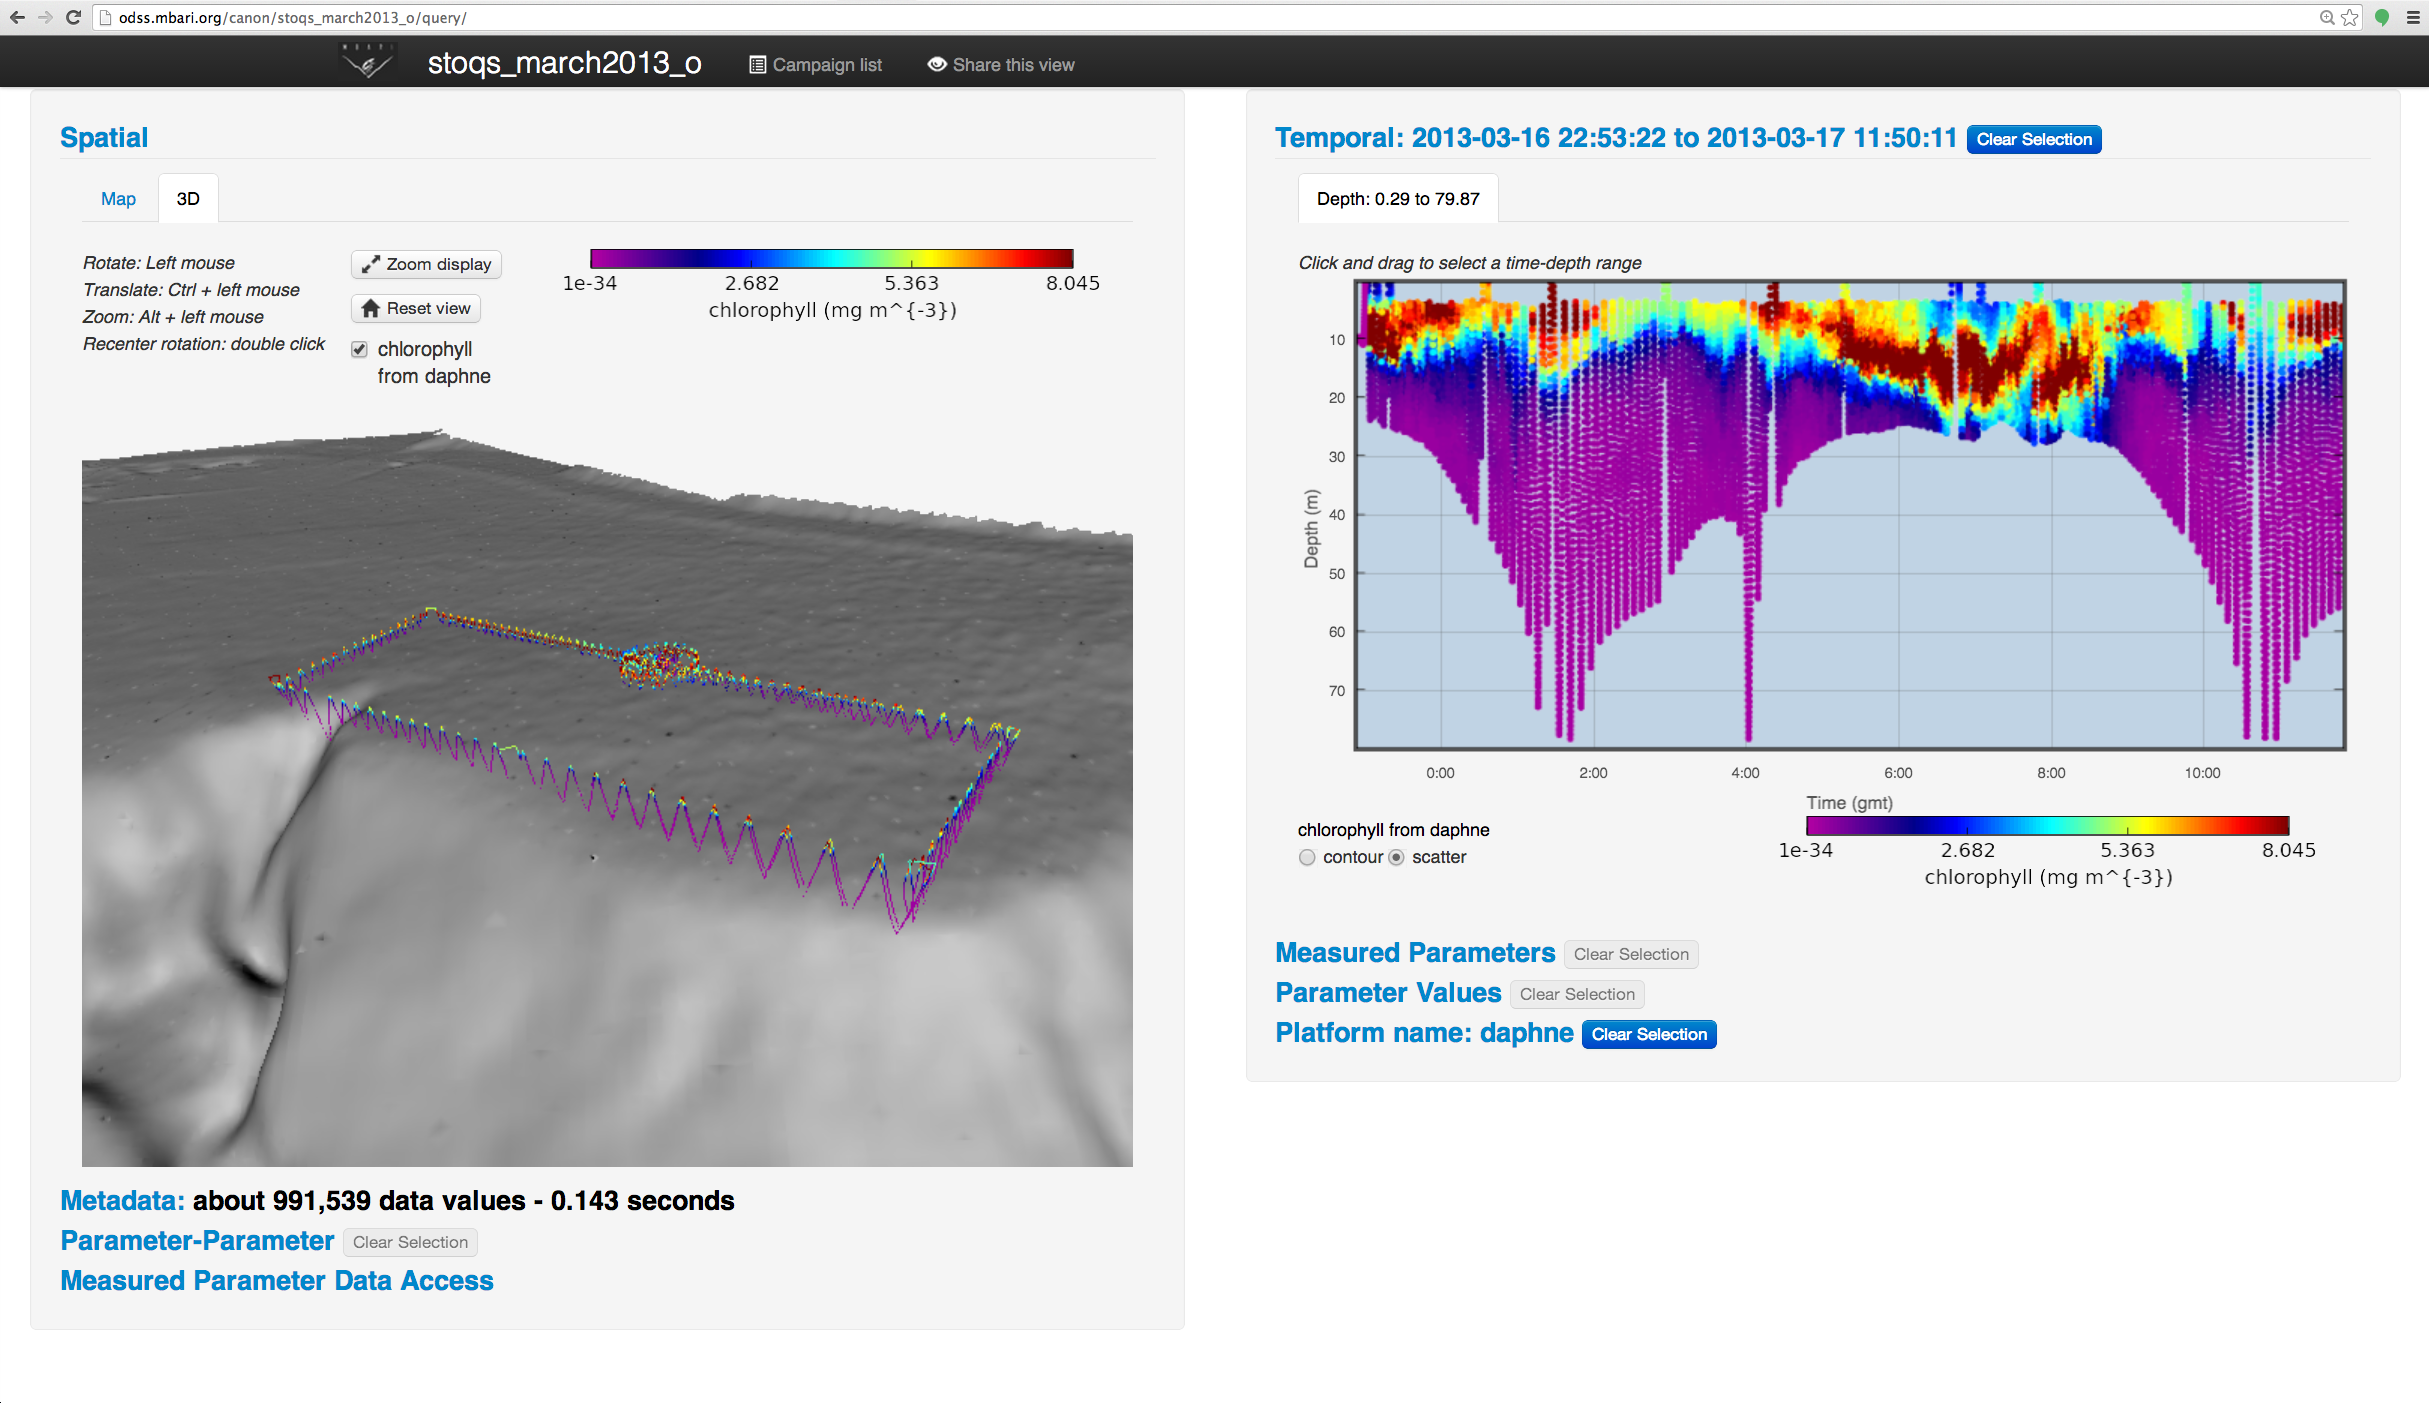
\includegraphics[width=6.4in]{STOQSUIscreencapture.png}
\caption{Screen capture of the STOQS web application showing underwater sensor data off the coast of southern California.}
\label{fig:STOQSscreen_capture}
\end{figure*}

The STOQS user interface displays a map of the vehicle tracks and a time series of depth profiles of the vehicles (Fig.~\ref{fig:STOQSscreen_capture}). Any of items in the right hand panel may be selected, which initiates instant update of the other items that may be selected. With this faceted search capability the user can quickly narrow a selection for data of interest. For instance in Fig.~\ref{fig:STOQSscreen_capture} the platform "daphne"  and a time range of about a half a day have been selected. The interface is reactive to browser screen size and behaves appropriately when viewed on tablets and smart phones.

Within the web application data are retrieved directly from the database via AJAX (Asynchronous JavaScript and XML) requests delivering data in JSON (JavaScript Object Notation) data structures. Client-side JavaScript code can then format these data as needed for display in the web page. Any DOM (Document Model Object) element, such as buttons and checkbox labels, and 2D plot can be updated with data from the database. In fact, requested data can update any DOM element, including elements in the 2D plotting library FLOT an in an X3D scene graph. 




\section{X3D Integration}

Data ret
X3D is ideally suited for building visualizations of all manner of real-world objects and information constructs in a geospatial context.  



Section 2 of this paper presents a specific solution to the problem with GeoOrigin.


\section{Terrain Rendering}

\subsection{GeoElevationGrid}

\subsection{POPGeometry in GeoCentric coordinates}

\begin{itemize}
\item Create point cloud .asc file with 10x vertical exaggeration:
\begin{verbatim}
grd2xyz Monterey25.grd --D_FORMAT=%f | \
  sed '/NaN/d' | \
  awk '{print $1, $2, 10 * $3}' | \ 
  mapproject -E --D_FORMAT=%f > \
  Monterey25_10x.asc
\end{verbatim}
\item Process in Meslab:
\begin{itemize}
\item Load .asc file
\item Point Sets - Compute normals for point sets
\item Surface Reconstruction: Poisson (Octree Depth: 12, Solver Divide: 10)
\item Remeshing, Simplification and Reconstruction - Quadric Edge Collapse Decimation:
\begin{itemize}
\item Target number of faces: 1,500,000 
\item Preserve Normal
\item Preseve Topology
\item Optimal Position of Simplified Vertices
\item Planar Simplification
\item Post-simplification cleaning
\end{itemize}
\item Cleanup (with plenty of intermediate saves)
\item Smoothing� - Laplacian smooth (surface preserve)
\item Export mesh to .ply
\end{itemize}
Some statistics on performance�.

\end{itemize}



% Prevent hyphenation
\hyphenation{GeoLOD}
\hyphenation{GeoTerrainLOD}

\section{Discussion}

\section{Conclusion}

Initial experiments with integrating X3D with a data drive web application have proven quite successful. The capability that X3DOM provides for updating scene graph elements with data from a database opens many possibilities for visualizing data. 


\section*{Acknowledgements}

Development of STOQS has been supported by the David and Lucile Packard Foundation; it is an open source software project built upon a framework of free and open source software and is available for anyone to use. For more information please see: http://code.google.com/p/stoqs/.




\bibliographystyle{acmsiggraph}
\nocite{*}
\bibliography{IntegrationOfX3DGeospatial}




\end{document}
